\section{Generative Adversarial Networks}\label{sec:GAN}
Generative Adversarial Networks (GANs)~\cite{} are a type of generative model
that uses a minimax algorithm to generate images. The network is composed of
multiple parts: a generator and a discriminator, as shown in
Figure~\ref{fig:gan}. The generator takes as input some noise from a known
distribution and then the generator upscales that into the size of the desired
data while also trying to match the data. The discriminator takes two different
types of inputs and tries to distinguish between the two, real data as well as
data from the generator.

\begin{figure}[ht]
    \centering
    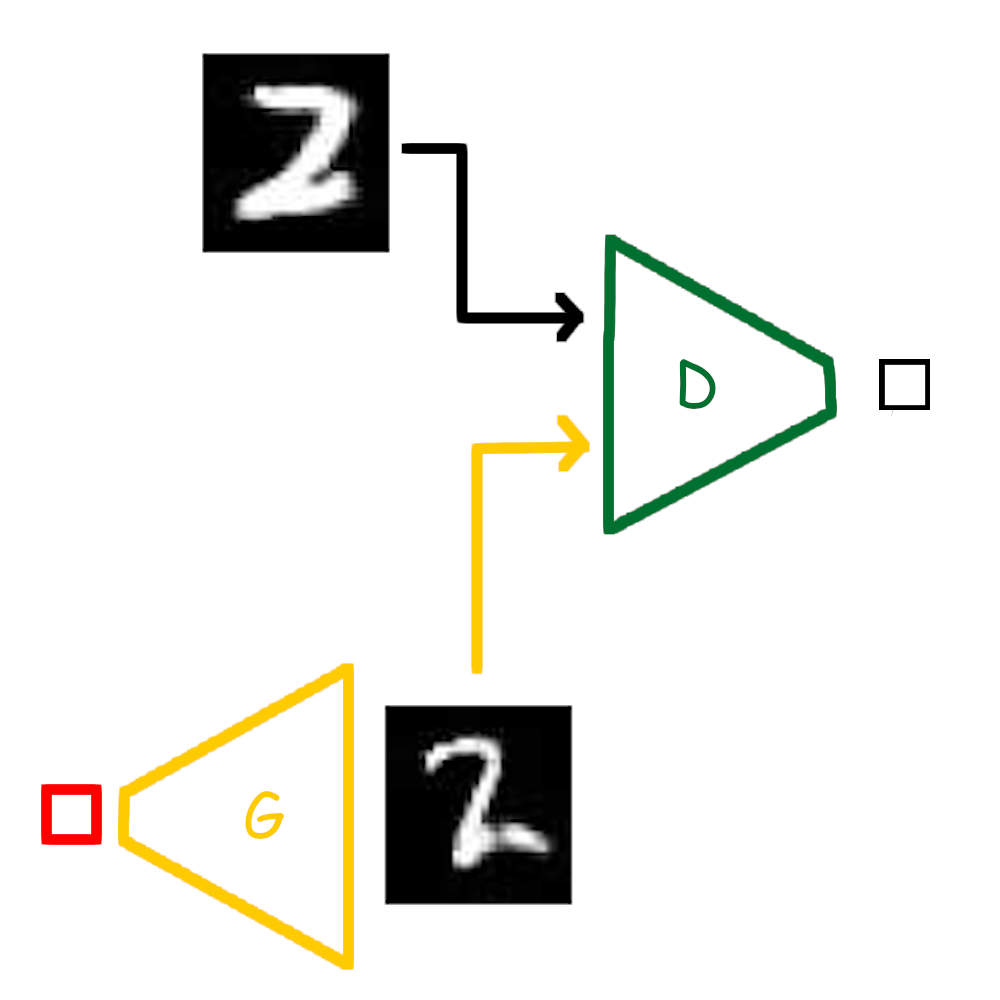
\includegraphics[width=0.48\textwidth]{GAN.png}
    \caption{A Generative Network where G represents the generator and D represents
        the discriminator.}
    \label{fig:gan}
\end{figure}

To train this network one trains the discriminator first, then the generator,
and then repeats the process. The goal is to make sure that the discriminator
can easily tell the difference between real and generated images. Then the
generator needs to be trained up to the point where it can fool the
discriminator. By doing this dual cycle eventually the generated data become so
good that the discriminator cannot be further improved by training. 

GANs are extremely popular in generative research because their ability to
produce high quality images. But because they are implicit density estimators
they have a few limitations. Because they do not learn the density function it
is more difficult to infer between different images, for example: someone
wearing glasses and someone not. Being able to infer this allows one to augment
an image to add the new feature. While there is plenty of research where people
have figured out how to solve these types of problems with GANs~\cite{} they do
not perform this action by direct inference like explicit density estimators do.
By looking at the latent space of a typical GAN, Figure~\ref{fig:ganLS}, we can
see that there is not a clear clustering of like features.

\begin{figure}[ht]
\centering
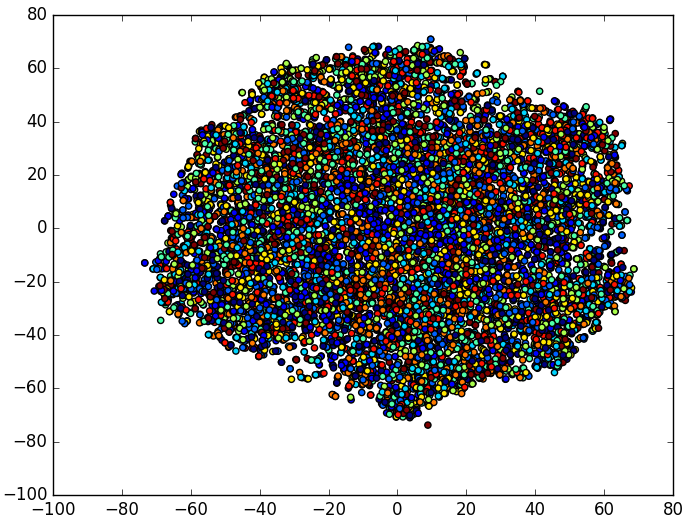
\includegraphics[width=0.48\textwidth]{GANLatent.png}
\caption{Latent space of a typical GAN}
\label{fig:ganLS}
\end{figure}

%\subsection{ClusterGAN}
%ClusterGAN~\cite{} tries to solve the problem of poor interpretability in the latent
%space. By doing this, ClusterGAN can allow GANs to perform a version of
%representation learning, or allowing the model to disentangle hidden features
%and semantics in the data. To accomplish this they use a mixture of discrete and
%continuous latent variables, use a novel backpropagation algorithm, and a
%clustering specific loss function. 
%
%For the discrete and continuous mixture of data they sample from normal random
%variables as well as one-hot encoded vectors. By modifying the standard
%deviation they can ensure that the latent space separates. 
%
%\textbf{TODO}

\subsection{StyleGAN}
StyleGAN is a popular state of the art GAN architecture that produces
impressively good images. One of the drawbacks of GANs is that they frequently
have "monsters", blobs, and phase errors. An example of the blobs is shown in
Figure~\ref{fig:blobs}. GAN monsters are grotesque looking creations that
generally take on features like the intended but with extra features. For
example a GAN generated cat may have a head disassociated from its body or a GAN
face could have a mouth where an eye should be. The third type of problem they
solved is a phasing issue. A common example of this is how teeth will align
forward while a head may be looking in a different direction.

\begin{figure}[ht]
\centering
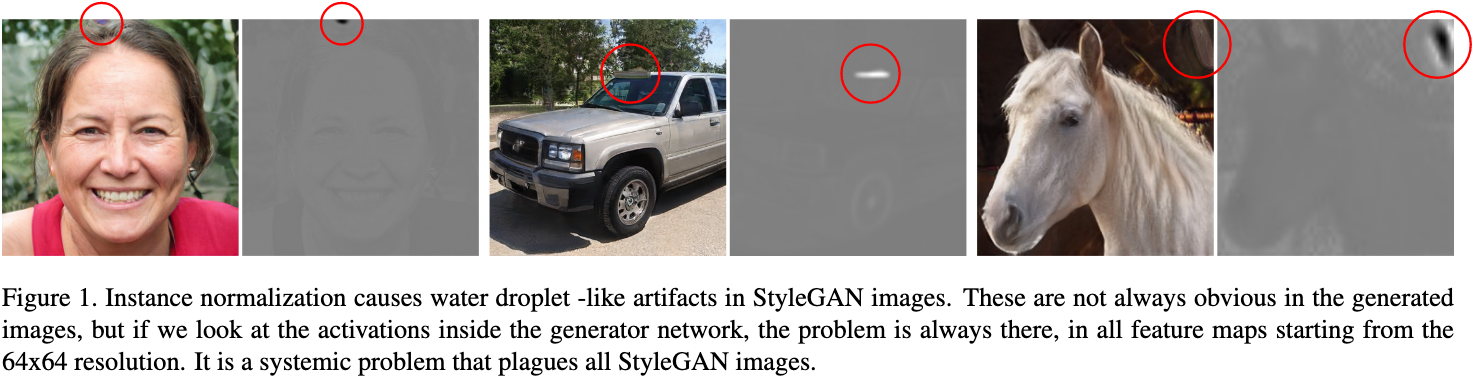
\includegraphics[width=0.48\textwidth]{StyleGAN2_blobs.png}
\caption{GAN blobs from StyleGAN}
\label{fig:blobs}
\end{figure}

StyleGAN2 solves this problem with a few changes to their original work. To
reduce the instances of monsters they introduced a perceptual path length (PPL)
regularizer. They introduced this because they noticed that images with higher
quality had lower PPL scores. By introducing this regularizer they can ensure
that the generated images will have minimized PPL. In a change of pace from
conventional GAN architectures, StyleGAN2 used skip generators and a residual
discriminator to replace progressive growing. They also introduced lazy
regularization, where they split the loss and regularization terms, and they
regularize every 16 minibatches. Finally, StyleGAN2 doubled the size of the
output images, to 1024x1024, greatly increasing the resolution of generated
images. With all these improvements StyleGAN2 was able to generate unprecedented
high quality images, improving as much as 30\% from StyleGAN, a work done only a
year earlier. 
